\documentclass[letterpaper,twocolumn,10pt]{article}
\usepackage{usenix}
\usepackage{mathptmx}
\usepackage[colorlinks,linkcolor=red,anchorcolor=blue,citecolor=green,urlcolor=black]{hyperref}
\usepackage{subfigure}
\usepackage{epsfig}
\usepackage{multirow}
\usepackage{array}
\usepackage{breqn}
\usepackage{pgfplots}
\usepackage{pgfplotstable}
\usepackage{sansmath}
\usepackage{booktabs}
\pgfplotsset{compat=1.5}
\DeclareGraphicsExtensions{.pdf}


\newcommand{\comments}[1]{}

%pgfplots setup
\pgfplotsset{
    %You are supposed to use append style rather than just setting
    %parameters globally so they are easier to override to special cases
    %thickness options:thin,ultra thin,very thin,semithick,thick,very thick
    every axis/.append style={
        thick,
        tick style={thick},
        tick label style={font=\small\mathversion{sans}\sffamily},
        label style={font=\small\sffamily},
        font={\small\sffamily},
        mark size=1.0
    },
    every legend/.append style={font={\small\mathversion{sans}\sffamily}}
}
\pgfplotsset{
    every mark/.append style={solid}
}
\pgfplotscreateplotcyclelist{mcolor}{%
    {blue,every mark/.append style={fill=blue},mark=*},
    {red,every mark/.append style={fill=red},mark=square*},
    {brown,every mark/.append style={fill=brown},mark=triangle*,mark size=1.5},
    {black,every mark/.append style={fill=black},mark=diamond*,mark size=1.5},
    {green!60!black,every mark/.append style={fill=green!60!black},mark=pentagon*,mark size=1.4},
    {magenta!90!black,every mark/.append style={fill=magenta!90!black},mark=star,mark size=1.5},
    {densely dashed,blue,every mark/.append style={fill=blue},mark=*},
    {densely dashed,red,every mark/.append style={fill=red},mark=square*},
    {densely dashed,brown,every mark/.append style={fill=brown},mark=triangle*,mark size=1.5},
    {densely dashed,black,every mark/.append style={fill=black},mark=diamond*,mark size=1.5},
    {densely dashed,green!60!black,every mark/.append style={fill=green!60!black},mark=pentagon*,mark size=1.4},
    {densely dashed,magenta!90!black,every mark/.append style={fill=magenta!90!black},mark=star,mark size=1.5}}

\pgfplotscreateplotcyclelist{mmark*}{
    {mark=*},
    {mark=square*},
    {mark=triangle*,mark size=1.5},
    {mark=diamond*,mark size=1.5},
    {mark=pentagon*,mark size=1.4},
    {mark=star,mark size=1.5},
    {mark=asterisk,mark size=1.5},
    {mark=+,mark size=1.5},
    {mark=Mercedes star,mark size=1.5}}

\pgfplotscreateplotcyclelist{mline}{
    {solid,blue,every mark/.append style={fill=blue}},
    {densely dashed,red,every mark/.append style={fill=red}},
    {densely dotted,brown,every mark/.append style={fill=brown}},
    {loosely dotted,black,every mark/.append style={fill=black}},
    {loosely dashed,green!60!black,every mark/.append style={fill=green!60!black}},
    {densely dashdotted,magenta!90!black,every mark/.append style={fill=magenta!90!black}},
    {densely dashdotdotted,teal,every mark/.append style={fill=teal}},
    {loosely dashdotted,orange,every mark/.append style={fill=orange}},
    {loosely dashdotdotted,violet,every mark/.append style={fill=violet}}}

    \pgfplotsset{cycle list name=mcolor}

\begin{document}

%\title{Collocated Deduplication with Fault Isolation for Virtual Machine Snapshot Backup [draft]}
\title{
Collocated Snapshot Backup with VM-Centric Deduplication in the Cloud}
\author{
  Wei Zhang$^{\star}$, Michael Agun$^\star$, Tao Yang$^\star$, and Hong Tang$^\dagger$ \\
  {\normalsize$^\star$  University of California at Santa Barbara}, {\normalsize$^\dagger$Alibaba Inc.} \\
  \{wei, tyang, dagun\}@cs.ucsb.edu, hongtang@alibaba-inc.com
}

\maketitle

\begin{abstract}
A cloud environment that hosts a large number of virtual machines (VMs) has
a high storage demand for frequent backup of system image snapshots. 
Deduplication of data blocks is necessary to eliminate
redundant blocks and reduce cost. Collocating a cluster-based duplicate service with other cloud services
reduces network traffic;
however, performng global deduplication and letting a data block be shared
by many virtual machines is resource expensive and less fault-resilient. 
This paper proposes a VM-centric collocated backup service that  
localizes deduplication as much as possible within each virtual machine using similarity-guided
search and associates  underlying file blocks with one VM for most cases.
It restricts global deduplication to popular blocks with extra replication support.
Our analysis shows that  this VM centric scheme 
can  provide  better fault tolerance while using a small amount of computing and storage resources. 
This  paper  describes a comparative evaluation of this scheme in  accomplishing a competitive deduplication 
efficiency while sustaining a good backup throughput. 
\end{abstract}

\section{Introduction}
In a cluster-based cloud environment,
each physical machine runs a number  of virtual machines as  instances of a guest operating system 
and their  virtual hard disks are represented as virtual disk image files in the host operating system.
Frequent  snapshot backup of virtual disk images  can increase  the service reliability. 
For example, the Aliyun cloud, which is  the largest cloud service provider by Alibaba in China, 
automatically conducts  the backup of virtual disk images to all active users every day.
The cost of supporting a large number of concurrent backup streams is high
because of the huge storage demand. 
Using a separate  backup service with full deduplication support~\cite{venti02,bottleneck08}
can effectively identify and remove content duplicates among snapshots, 
but such a solution can be expensive. There is also a large amount of 
network traffic to transfer  data from the host machines to the backup facility
before duplicates are removed.

This paper seeks for a low-cost architecture option  that collocates
a backup service with other cloud services and  uses a minimum amount of resources. 
We also consider the fact that after
deduplication, most data chunks are shared by several to many virtual machines.
Failure of a few shared data chunks can have a 
broad effect and many
snapshots of virtual machines could be affected.
The previous work in deduplication focuses on the efficiency and approximation of
fingerprint comparison, and has not addressed fault tolerance issues  together with deduplication.
Thus we also seek deduplication options that yield better fault isolation.
Another issue considered is that
that garbage collection after deletion of old snapshots also competes for computing resources. 
Sharing of data chunks among by multiple VMs needs to be detected during
garbage collection and such dependencies complicate deletion operations. 

The key contribution is the development and analysis of a VM-centric approach
which considers fault isolation and integrates  multiple duplicate detection strategies
supported by similarity guided local deduplication
and popularity guided global deduplication. 
This approach localizes duplicate detection within each VM  
and packages only data chunks from the same VM into a file system block as much as possible.
By narrowing duplicate sharing within a small percent of common data chunks and exploiting their popularity,
this scheme can afford to allocate extra replicas of these shared chunks for better
fault resilience while sustaining competitive deduplication efficiency.
In addition, our VM-centric design allows garbage collection to be performed in a localized
scope and we propose an approximate deletion scheme to reduce this cost further.
Localization also brings the benefits of greater ability to exploit parallelism so
backup operations can run simultaneously without a central  bottleneck.
This VM-centric solution uses a small amount of  memory while delivering reasonable deduplication efficiency. 

We have developed a prototype system that runs a cluster of Linux machines with Xen and uses 
a standard distributed file system for the backup storage. 

%************** Paper sections summary
%THIS NEEDS MODIFICATION
The rest of this paper is organized as follows.
Section~\ref{sect:background} reviews the background and discusses the  design options for snapshot backup 
with a VM-centric approach. 
Section~\ref{sect:deduplication}  analyzes the tradeoff and benefits of our approach. 
Section~\ref{sect:architecture}  describes our system architecture and implementation details.
%   the benefit of our approach for fault isolation. 
Section~\ref{sect:evaluation} is our experimental evaluation that compares with other approaches.
Section~\ref{sect:conclusion}  concludes this paper.

\section{Background and Design Considerations}
\label{sect:background}
At a cloud cluster node, each instance of a guest operating system runs on a virtual machine, accessing virtual hard disks 
represented as virtual disk image files in the host operating system.
For VM snapshot backup, file-level semantics are normally not provided.
Snapshot operations take place at the virtual device driver level, which
means no fine-grained file system metadata can be used to determine the changed data. 
Backup systems have been developed to use content fingerprints to identify duplicate
content~\cite{venti02,Rhea2008}.  
As discussed earlier, collocating a backup service on the existing
cloud cluster avoids the extra cost to acquire a dedicated backup facility
and reduces the network bandwidth consumption in transferring the
raw data for backup. 
Figure~\ref{fig:collocated} illustrates the cluster architecture where
each physical machine runs a backup service and a distributed file system (DFS)~\cite{googlefs03,hdfs10} 
serves a backup store  for the snapshots.

\begin{figure}[htb]
    \centering
    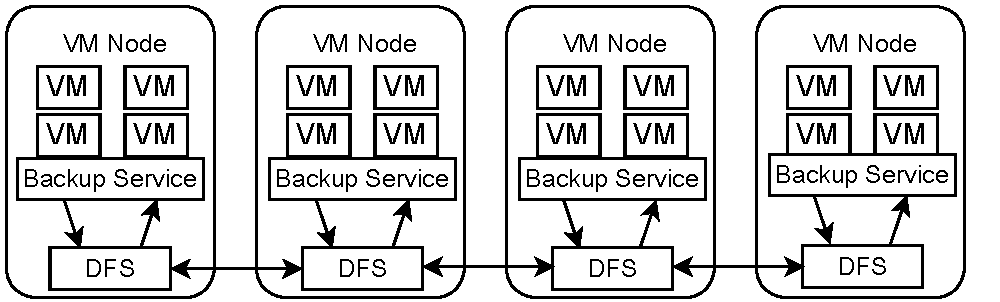
\includegraphics[width=3in]{images/colocated-arch}
    \caption{Collocated VM Backup System.}
    \label{fig:collocated}
\end{figure}

Since it is expensive to compare a large number of chunk signatures for deduplication,
several techniques have been proposed to speedup searching of duplicate
fingerprints. For example, the data domain method ~\cite{bottleneck08} 
uses  an in-memory Bloom filter and a prefetching cache for data chunks  which may be
accessed.  An improvement to this work with parallelization is in ~\cite{MAD210,DEBAR}.
The approximation techniques are studied in~\cite{extreme_binning09,Guo2011,WeiZhangIEEE}  
to reduce memory requirements with the tradeoff of a reduced deduplication ratio.
Additional inline deduplication techniques are studied in ~\cite{sparseindex09,Guo2011,Srinivasan2012}
and a parallel batch solution for cluster-based deduplication is 
studied in ~\cite{wei2013}. 
All of the above approaches have focused on optimization of deduplication
efficiency, and none of them have considered the impact
of deduplication on fault tolerance in the cluster-based environment that we have considered
in this paper.

Our key design consideration is VM dependence minimization during deduplication and file system block management.
\begin{itemize}
\item {\em Deduplication localization.}
Because a data chunk is compared with signatures collected from all VMs during
the deduplication process, only one copy of duplicates is stored in the storage,
this artificially creates data dependencies among different VM users. 
Content sharing via deduplication affects fault isolation since machine failures happen periodically 
in a large-scale cloud and
loss of a small number of shared data chunks can 
cause the unavailability of snapshots for a large number of virtual machines.
Localizing the impact of deduplication can increase fault isolation and resilience.
Thus from the fault tolerance point of view,  duplicate sharing among multiple VMs is 
discouraged. 
Another disadvantage of sharing is that it complicates snapshot deletion, 
which  occurs frequently when snapshots expire regularly. 
The mark-and-sweep approach~\cite{Guo2011} is effective for deletion, but has a high cost, and its main cost
is to count if a data chunk is still shared by other snapshots.
Localizing deduplication can  minimize data sharing and simplify deletion while sacrificing 
deduplication efficiency, and  can facilitate parallel execution of snapshot operations.
\item{\em  Management of file system blocks.}
The file system block (FSB) size in a distributed file system such as  Hadoop and GFS is uniform and large (e.g.  64MB),
while the data chunk in a typical deduplication system is of a non-uniform size with 4KB or 8KB on average.
Packaging data chunks to an FSB can create more data dependencies among VMs
since a file system block can be shared by even more VMs.
Thus we need to consider a minimum association of FSBs to VMs in the packaging process.
\end{itemize}

Another consideration is the computing cost of deduplication.
Because of collocation of this snapshot service with other existing cloud services, 
cloud providers will want the backup service to only consume small resources
with a minimal impact to the existing cloud services.
The key resource for signature comparison  is memory for storing the fingerprints. 
We will consider the approximation techniques with reduced memory consumption along 
with the fault isolation considerations discussed below. 

We call the traditional deduplication approach as   VM-oblivious (VO)
because they compare fingerprints of snapshots without consideration of VMs.
With the above  considerations in mind, we study a 
VM-centric approach (called VC)
for a collocated backup service with resource usage friendly
to the existing applications.  

In designing a VC duplication algorithm, we have considered and adopted some of
the following previously-developed techniques.
1)
{\em Version-based change detection}.
VM snapshots can be  backed up  incrementally by identifying file segments that have
changed from the previous version of the snapshot~\cite{Clements2009,Vrable2009,TanIPDPS2011}.
Such a scheme  is  VM-centric since deduplication is localized. 
We are seeking for a tradeoff since 
global signature comparison can deliver additional compression~\cite{Guo2011,Dong2011,extreme_binning09}.
2) {\em Stateless  data Routing}.
One approach for scalable duplicate comparison is to use a content-based hash
partitioning algorithm called stateless data routing by Dong et al.~\cite{Dong2011} 
Stateless data routing divides the deduplication work with a similarity approximation. This work 
is similar to Extreme Binning by Bhagwat et al.~\cite{extreme_binning09} and 
each request is routed  to a machine which holds
a Bloom filter  or can fetch on-disk index for additional comparison.
While this approach is VM-oblivious, it motivates us to  use  a combined signature of a dataset to narrow
VM-specific local search.
3) {\em Sampled Index}.
One effective approach that reduces memory usage is 
to use a sampled index with prefetching, proposed  by Guo and Efstathopoulos\cite{Guo2011}. 
The algorithm is VM oblivious and it is not easy  to adopt for a distributed architecture. 
To use a distributed memory version of the sampled index, every deduplication request
may access a remote machine for index lookup and the overall overhead of access latency for all requests
can be significant.  


We will first discuss and analyze the integration of the VM-centric deduplication strategies with fault isolation, 
and then present
an architecture and implementation design with deletion support.

\section{VM-centric Snapshot Deduplication}
\label{sect:deduplication}

\subsection{Key VC  Strategies}
\label{sect:vc-strategies}
%\begin{itemize}
%\item 
\textbf{VM-specific local duplicate search within similar segments.}
We start with the changed block tracking approach in a coarse grain segment level.
In our implementation with Xen on an Alibaba platform, the segment size is 2MB
and the device driver is extended to support tracking changed segments using a dirty bitmap. 
Since every write for a segment will touch a dirty bit, the device driver maintains dirty bits in memory
and cannot afford a small segment size.
It should be noted that dirtybit tracking is supported or can be easily implemented in 
major virtualization solution vendors. For example,
the VMWare hypervisor has an API to let external backup applications know 
the changed areas since last backup. 
The Microsoft SDK provides an API that allows external applications to monitor 
the VM's I/O traffic and implement such changed block tracking feature.

\begin{figure}[htbp]
  \centering
  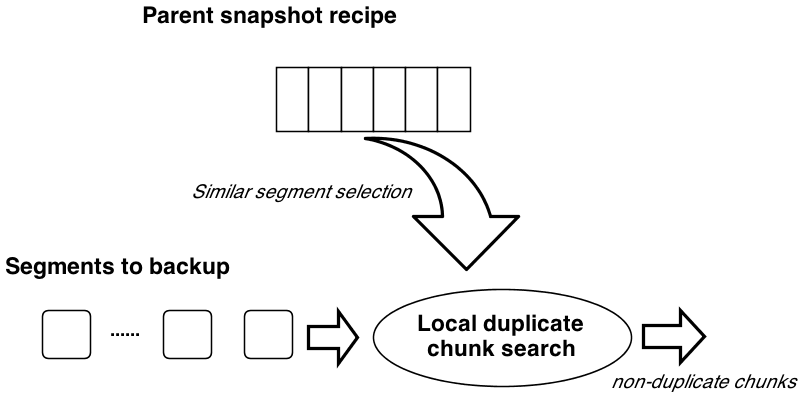
\epsfig{file=images/mh_local_dedup.png, width=3in}
  \caption{Similarity-guided local duplicate detection}
  \label{fig:local_dedup}
\end{figure}

Since the best deduplication uses a nonuniform chunk size 
in the average of 4K or 8K~\cite{Jin2009},
we conduct additional local similary guided deduplication on a snapshot by comparing
chunk fingerprints of a dirty segment 
with those in  {\em similar} segments from its parent snapshot. 
We define two segments are similar if their content signature is the same.
This segment content signature value is defined as the minimum value of all its chunk fingerprints 
computed during backup and is recorded in the snapshot metadata (called recipe). Note that this definition of
content similarity is an approximation~\cite{resemblance97}.  When processing a dirty segment,
its  similar segments can be found easily from the
parent snapshot recipe.  Then recipes of the similar segments are loaded to memory,
which contain chunk fingerpints to be compared.
To control the time cost of search, we set a limit on the the number of  similar segments recipes to be fetched. 
% Then,
%given a set of data chunks within a dirty segment,  we compare  these chunk fingerprints
%with those in similar segments.  
For a 2MB segment, its segment recipe is roughly 19KB which contains about 500 chunk fingerprints and other chunk metadata,
by limiting at most 10 similar segments to search, the amount of memory for maintaining those similar segment recipes is small.
As part of our local duplicate search we also compare the current segment
against the parent segment at the same offset.

%\item 
\textbf{Global deduplication with popular chunks and replication support.}
This step accomplishes the canonical global fingerprint lookup using a popular fingerprint index.
Our key observation is that the local deduplication has removed most of the duplicates.
There are fewer deduplication opportunities across VMs while the memory and network
consumption for global comparison is more expensive.
Thus our approximation is that the global fingerprint comparison only searches for the top $k$
most popular items. This dataset is called the \textbf{PDS} (popular data set). 
We define chunk popularity as the number of unique copies of the chunk in the data-store,
that is the number of copies of the chunk after local deduplication.
This number can be computed periodically (e.g., on a weekly basis).
Once the popularity of all data chunks is collected, the system only maintains the top $k$
most popular chunk fingerprints (called \textbf{PDS index}) in a distributed shared memory.  
Our previous work~\cite{WeiZhangIEEE} studies a preliminary solution using data popularity and this
paper improves this with a more comprehensive scheme with  similarity-guided search and fault isolation.

Since $k$ is relatively small and these top $k$ chunks are shared among multiple VMs, 
we can afford to provide extra replicas for these popular chunk data to enhance the fault resilience.

%\item 
\textbf{VM-centric file system block management.}
When a chunk is not detected as a duplicate to any existing chunk, this chunk will be written
to the file system. Since the backend file system typically uses a large block size such as 64MB, each VM will 
accumulate small local chunks. We manage this accumulation process using an log-structured storage scheme built
on a distributed file system discussed in Section~\ref{sect:architecture}.
%Non-PDS chunks from the same VM are stored in one append store. 
Each file system block is either dedicated to non-PDS chunks, or PDS-chunks.
A file system block for non-PDS chunks is associated with one VM and does not contain
any PDS chunks, such that our goal of fault isolation is maintained.
In addition, storing PDS chunks separately allows special replication handling for those popular shared data. 
%%% talk something about snapshot store advantage here? %%%

%The system allows all machines conduct backups in parallel, and each machine
%conducts the backup of one VM at a time, and thus only requires a write buffer for one VM.
%\end{itemize}

\begin{figure}
\centering
%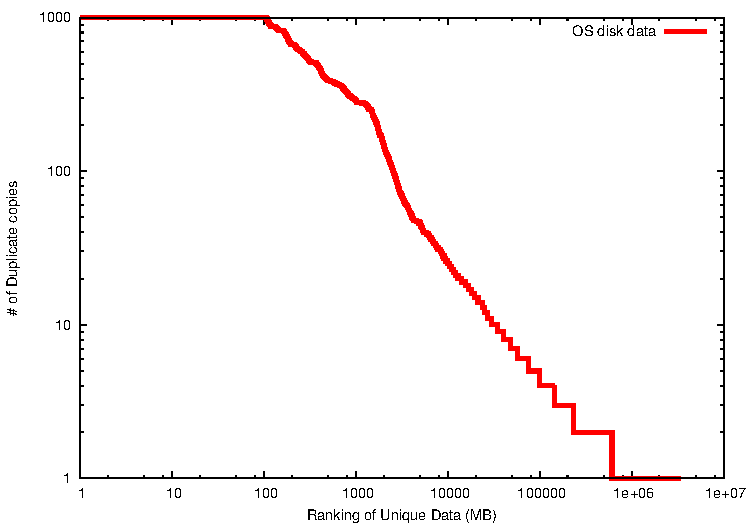
\epsfig{file=log-log.disk,width=3in}
%source ../vm_snapshot_sim/images/log-log.disk.eps
 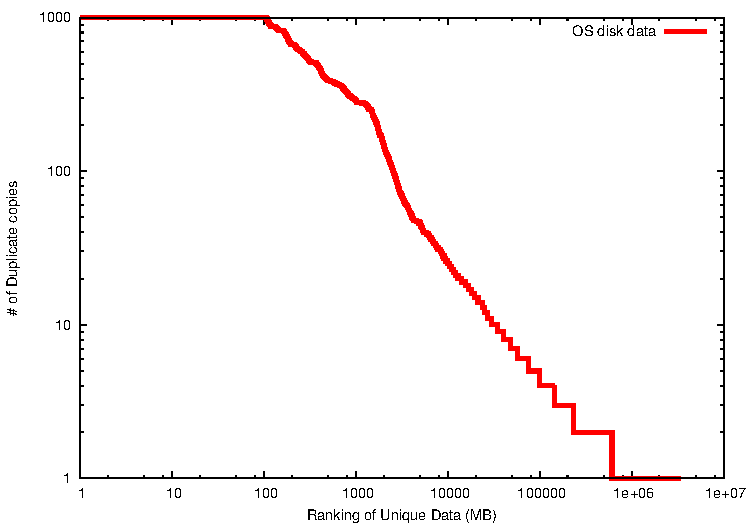
\includegraphics[width=3in]{figures/log-log-disk}
\caption{Duplicate frequency versus  chunk ranking in a log scale after local deduplication.}
\label{fig:Datazipf}
\end{figure}


% {\it [Need to find a place to put these numbers in: Total number of chunks 
% in 350 snapshots: 1,546,635,485. 
% Total number of chunks after localized dedup: 283,121,924. Total number of unique chunks: 87,692,682.]}
\subsection{Impact on deduplication efficiency}
Choosing the value $k$ for the most popular chunks affects the deduplication efficiency.
We analyze this impact based on the characteristics  of the VM snapshot traces
studied from  application datasets.
A previous study shows that the popularity of data chunks after local deduplication follows 
a Zipf-like distribution\cite{Breslau1999a} and its
exponent $\alpha$ is ranged between 0.65  and  0.7~\cite{WeiZhangIEEE}. 
Figure~\ref{fig:Datazipf} illustrates the Zipf-like distribution of chunk popularity.
The parameters we will use in our analysis below are defined in
Table~\ref{tab:symbol}. 

\begin{table}[htbp]
\centering
\begin{tabular}{|p{1.25cm}|p{5.5cm}|}
\hline
$k$ &  the number of top most popular chunks selected for deduplication\\ 
\hline
$c$ &  the total amount of data chunks in a cluster of VMs\\ 
\hline
$c_u$ &  the total amount of unique fingerprints after perfect  deduplication\\
\hline
$f_i$ &  the frequency for the $i$th most popular fingerprint\\
\hline
$\delta$ &  the percentage of duplicates detected in local deduplication\\
\hline
$\sigma$ & =$\frac{k}{c_u}$ which is  the percentage of unique data  belong to  PDS\\
\hline
$p$ & the number of machines in the cluster\\
% \hline
% $V$ & the average number of VMs hosted on each machine\\
\hline
$E$ & the deduplication efficiency of VC approach\\
%\hline
%$D$ & the amount of unique data on each machine\\
%\hline
%$C$ & the average data chunk size. Our setting is  4K.\\
%\hline
%$s$ & the average size of file system blocks in the distributed file system. The default is  64MB.\\
%\hline
%$m$ & memory size on each node used by VC\\ 
%\hline
%$E$ & the size of an popular data index entry\\
\hline
$N_1$ & the average number  of non-PDS file system blocks  in a VM for VC\\
\hline
$N_2$ & the average number  of PDS file system blocks  in a VM for VC\\
\hline
$N_o$ & the average number  of file system blocks  in a VM for VO\\
\hline
A(r) & the availability of a file system block with replication degree $r$\\
\hline
\end{tabular}
\caption{Modeling  parameters}
\label{tab:symbol}
\end{table}


%Table~\ref{tab:symbol} defines paramters $c$, $c_u$, $f_i$, and $\delta$ used below.
%let $c$ be the total number of data chunks. 
%$c_u$ be the total number of fingerprints 
%in the global index after complete deduplication, and
%$f_i$ be the frequency for the $i$th most popular fingerprint. 
By Zipf-like distribution, $f_i = {f_1}/{i^\alpha}.$
The total amount of chunks reside in our backup storage which
has local duplicates excluded is $c (1-\delta)$, this can be represented
as the sum of each unique fingerprint times its frequency:
%Since $ \sum_{i=1}^{c_u}f_i = c (1-\delta)$,
\[
f_1 \sum_{i=1}^{c_u}\frac{1}{i^\alpha} = c (1-\delta).
\]
Given $\alpha <1$, $f_1$ can be approximated with integration:
\begin{equation}
f_1=\frac{c(1-\alpha)(1-\delta)}{c_u^{1-\alpha}}.
\end{equation}

Thus putting the $k$ most popular fingerprints into PDS index can remove the following number of chunks during global 
deduplication:
\[
f_1 \sum_{i=1}^{k}\frac{1}{i^\alpha} \approx  
f_1 \int_{1}^{k}\frac{1}{x^\alpha} dx  \approx  f_1\frac{  k^{1-\alpha}} {1-\alpha}
=c(1-\delta) \sigma^{1-\alpha}.
\]

Deduplication efficiency of the VC approach using top $k$ popular chunks
is the percentage of duplicates that can be detected:  
\begin{equation}
\label{eq:dedupeff}
%\begin{split}
%e_k &= 
E=\frac{ c\delta + c(1-\delta) \sigma^{1-\alpha}}
{c  - c_u }.\\
%\end{split}
\end{equation}

% After the global deduplication, the number of remaining chunks is:
% \[
% c-E(c-c_u)
% \] 

We store the PDS index using a distributed shared memory hashtable such as Memcached
and allocate a fixed percentage of memory space per physical machine for top $k$ popular items.
As the number of physical machines ($p$) increases,
the entire cloud cluster can host more VMs; however,  ratio $\sigma$ which is $k/c_u$ remains
a constant because each physical machine on average still hosts a fixed constant number of 
VMs. Then the overall deduplication efficiency of VC defined in Formula~\ref{eq:dedupeff}
remains constant.
Thus the deduplication efficiency is stable  as $p$ increases as long as $\sigma$  is a constant.


\begin{figure}[htbp]
  \centering
    \begin{tikzpicture}
            \begin{axis}[
            %title={PDS Coverage},
            width=\linewidth,
            height=0.6\linewidth,
            cycle multi list={
                mline\nextlist
                [3 of]mmark*\nextlist
            },
            %cycle list name=mcolor,
            xlabel={Total num. chunks stored (in billions)},
            ylabel={PDS Coverage (\%)},
            %extra y ticks={4.5,5.5,6.5} %to add extra ticks
            mark options=solid,
            %legend pos=outer north east,
            legend columns=2,
            legend style={
                at={(0.5,-0.30)},
            anchor=north},
            ]
            \addplot table[x expr=\thisrow{InputChunks}/1000000000,y=A1] {figures/cds_coverage.txt};
            \addplot table[x expr=\thisrow{InputChunks}/1000000000,y=A2] {figures/cds_coverage.txt};
            \addplot table[x expr=\thisrow{InputChunks}/1000000000,y=A4] {figures/cds_coverage.txt};
            \addplot table[x expr=\thisrow{InputChunks}/1000000000,y=T1] {figures/cds_coverage.txt};
            \addplot table[x expr=\thisrow{InputChunks}/1000000000,y=T2] {figures/cds_coverage.txt};
            \addplot table[x expr=\thisrow{InputChunks}/1000000000,y=T4] {figures/cds_coverage.txt};
            \legend{Measured ($\sigma=1\%$),Measured ($\sigma=2\%$),Measured ($\sigma=4\%$),Predicted ($\sigma=1\%$),Predicted ($\sigma=2\%$),Predicted ($\sigma=4\%$)};
            \end{axis}
    \end{tikzpicture}
  \caption{Predicted vs. actual PDS coverage as data size increases.}
  \label{fig:cds-coverage}
\end{figure}
Ratio $\sigma^{1-\alpha}$ represents the percentage of the remaining
chunks detected as duplicates in global deduplication due to PDS.
We call this PDS coverage.
Figure~\ref{fig:cds-coverage} shows predicted PDS coverage using $\sigma^{1-\alpha}$ when $\alpha$ is fixed at
0.65 and measured PDS coverage in our test dataset.
$\sigma=2\%$ represents memory usage of approximately 100MB memory per machine for the PDS.
While the predicted value remains flat, the  real coverage actually increases as the data size
increases, which indicates that $\alpha$ increases with the data size. 
Therefore in practice, the coverage of the PDS increases as more VMs are involved.

\subsection{ Impact on Storage Space and Fault Isolation}
 
\begin{figure}
    \centering
    \subfigure[Sharing of file blocks under VC]
    {
        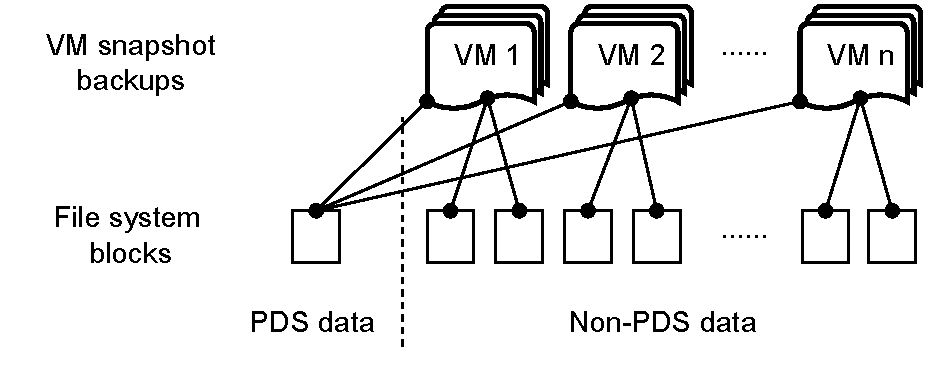
\includegraphics[width=3in]{images/share_vc}
        \label{fig:share_vc}
    }
    \\
    \subfigure[Sharing of file blocks under VO]
    {
        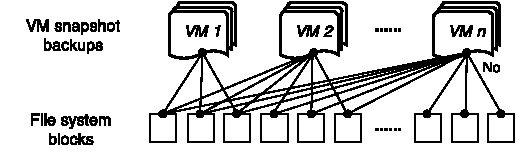
\includegraphics[width=3in]{images/share_vo}
        \label{fig:share_vo}
    }
    \caption{Bipartite association of VMs and file blocks under (a) VC and (b) VO. }
    \label{fig:share}
\end{figure}

The replication degree of the backup storage 
is $r$ for regular file blocks and $r=3$ is a typical setting in distributed
file systems~\cite{googlefs03,hdfs10}.
In the VC approach, a special replication degree $r_c$ is used for PDS data where $r_c>r$. 
The storage cost for VO with full deduplication is $c_u *r$ and for VC, it is
$ k*r_c  + (c-E(c-c_u))*r$. Thus The storage cost ratio of $VC$ over $VO$ is 
\[
\sigma \frac{r_c}{r} + \frac{c-e(c-c_u)}{c_u}.
\]
Since $\sigma$ is small (it is 2\% in our experiments),  
term $\sigma \frac{r_c}{r}$ is small in the above expression.  
Thus the impact on storage increase is very small even when we choose a large $r_c/r$ ratio. 
For example, $r_c/r=2$ or 3. 

Next we  assess  the impact of losing $d$ machines 
to the the VC and VO approaches.  
A large $r_c/r$ ratio can have a positive impact on full availability of VM snapshot blocks.
We use file system blocks rather than a deduplication
data chunk as our unit of failure because the DFS keeps
filesystem blocks as its base unit of storage.
To compute the full availability of all snapshots of a VM, we derive
the probablity of losing a snapshot file block of a VM by
estimating the number of file system blocks per VM in each approach.
As illustrated in Figure~\ref{fig:share},
we build a bipartite graph representing the association from unique file system blocks
to their corresponding VMs in each approach. An association edge is  drawn  from a file block  to a VM 
if this block is used by the VM. 

For VC, each VM has an average number of $N_1$ non-PDS file system blocks
and  has  an average of  $N_2$ PDS file system blocks. 
Each non-PDS file system block is associated with one VM
 and  we denote that PDS file system blocks are
shared by an average of $V_c$ VMs. Let $s$ be the average number of chunks per file block, 
$V$ be the average number of VMs hosted on each machine. Then, 
\[
V *p*N_1 *s  \approx c-E(c-c_u)\; \mbox{ and } \; 
V *p*N_2 *s  \approx c_u \sigma V_c.
\]

For VO, each VM has an average of $N_o$ file system blocks
and let $V_o$ be the average number of VMs shared by each file system block.
\[
V *p*N_o *s  = c_u  V_o.
\]

Since each file block (with default size $64MB$) contains many chunks (on average 4KB),
each file block contains the hot low-level chunks shared by many VMs, and it also contains
rare chunks which are not shared.  From the above equations:
\[
\frac{N_1}{N_o} \approx  \frac{c-E(c-c_u)}{c_uV_o}.
\] 

If we achieve very high deduplication efficiecny, then $N_1$ would be much smaller than $N_o$. 
When there is a failure in file blocks with replication degree $r$
and there is no failure for PDS data with more replicas,   a VM in
the VC approach has a much lower chance to lose a snapshot than VO. 
%Figure~\ref{fig:fsb-links} shows the average number of VMs sharing each file block from
%our test dataset.
%For VC, we only show
%the sharing degree of  PDS-oriented file blocs  because non-PDS blocks always belong to
%one VM.
%Figure~\ref{fig:fsb-links} shows the average number of VMs sharing each file block from our test data.
Figure~\ref{fig:vm-links} shows the average number of file system blocks for each VM in VC and in VO. 
From data, we have observed that $N_1 +N_2 < N_o$ in practice. 
This is likely because the PDS FSBs tightly pack data used by many VMs, 
which decreases the overall number of FSBs required to backup a VM.
Note that  if  the backup for multiple VMs were conducted concurrently, there could be many more
VMs sharing each file block on average in VO. 

%Therefore, even when there is a loss of a PDS block, the VC approach tolerates the fault better.

\comments{
\begin{figure}[htbp]
  \centering
	\begin{tikzpicture}
		\begin{axis}[
                width=\linewidth,
                height=0.6\linewidth,
		%title={VO FSB links},
		xlabel={Number of VMs},
		ylabel={Avg. Num. VMs sharing FSB},
                cycle list name=mline,
                xmin=0,
                ymin=0,
                xmax=106,
		%extra y ticks={4.5,5.5,6.5} %to show extra ticks
		legend pos=north west
		]
                \addplot table[x=VMs,y=FSBLinks] {figures/vo_fsb_links_105.txt};
		\addplot table[x=VMs,y=cdslinks] {figures/cds_links_105.txt};
                \legend{VO, PDS in VC};
		\end{axis}
	\end{tikzpicture}
  \caption{Measured average number of VMs sharing a 64MB FSB in VO and in VC.}
  \label{fig:fsb-links}
\end{figure}

}

\begin{figure}[htbp]
  \centering
	\begin{tikzpicture}
		\begin{axis}[
		%title={VO VM links},
                width=\linewidth,
                height=0.6\linewidth,
		xlabel={Number of VMs},
		ylabel={Avg. Num. FSBs used by VM},
                xmin=0,
                ymin=0,
                xmax=106,
		%extra y ticks={4.5,5.5,6.5} %to show extra ticks
		legend pos=south west
		]
                \addplot[blue,mark=none] table[x=VMs,y=N_O] {figures/vm_links_all.txt};
                %\addplot[red,dotted,mark=none] table[x=VMs,y expr=\thisrow{N_1}+\thisrow{N_2}] {figures/vm_links_all.txt};
                \addplot[red,dashdotted] table[x=VMs,y=N_1] {figures/vm_links_all.txt};
                \addplot[red,densely dashed,mark=none] table[x=VMs,y=N_2] {figures/vm_links_all.txt};
                \legend{$N_o$,
                    %$N_1+N_2$,
                    $N_1$,
                    $N_2$};
		\end{axis}
	\end{tikzpicture}
  \caption{Measured average number of 64MB FSBs used by a single VM. For VC both the number of PDS and Non-PDS FSBs used are shown.}
  \label{fig:vm-links}
\end{figure}

The full snapshot availability of a VM is estimated as follows with parameters $N_1$ and
 $N_2$ for VC and $N_o$ for VO.
Given normal data replication degree $r$, PDS data replication degree $r_c$, 
the availability of a file system block is the probability that  
all of its replicas do not appear in any group of $d$ failed machines among the total of $p$ machines. 
Namely, we define it as
\[
A(r) = 1-\binom{d}{r}/ \binom{p}{r}. 
\]
Then the availability of one VM's snapshot data under VO approach is the probability that
 all its file system blocks are unaffected during the system failure:
\begin{equation}
\label{eq:VO}
%(1-\frac{ \binom{d}{r}} { \binom{p}{r} })^{N_o}. 
A(r)^{N_o}. 
\end{equation}

For VC, there are two cases for $d$ failed machines.
\begin{itemize}
\item
When $r \le d<r_c$,  there is no PDS data loss and  
the full snapshot availability of a VM in the VC approach is 
\begin{equation}
\label{eq:VC1}
%(1-\frac{\binom{d}{r}} { \binom{p}{r} })^{N_1}.
A(r)^{N_1}.
\end{equation}
Since $N_1$ is typically much smaller than $N_o$, 
the VC approach has a higher availability of VM snapshots than VO.

\item
When $r_c \leq d$, both non-PDS and PDS file blocks in VC can have a loss.
The full snapshot availability of  a VM in the VC approach is
\begin{equation}
\label{eq:VC2}
% (1-\frac{ \binom{d}{r}} { \binom{p}{r} })^{N_1} 
% *
% (1-\frac{ \binom{d}{r_c}} { \binom{p}{r_c} })^{N_2}.
A(r)^{N_1} * A(r_c)^{N_2}
\end{equation}
Table~\ref{tab:fsb-availability} lists the $A(r)$ values with
%that the availability of an individual file system block
with different replication degrees. This demonstrates inequality 
% $1-\frac{ \binom{d}{r}} { \binom{p}{r} } < 1-\frac{ \binom{d}{r_c}} { \binom{p}{r_c} }$
$A(r) < A(r_c)$.  Since $N_1$ is much smaller than $N_o$ as discussed previously, 
these two conditions support that VC has a  higher availability. 
%comparing  Formula~\ref{eq:VO} and~\ref{eq:VC}. 
\end{itemize} 

\comments{
\begin{figure}[htbp]
  \centering
    \begin{tikzpicture}
            \begin{axis}[
                width=\linewidth,
                height=0.6\linewidth,
            %title={FSB Availability},
            cycle list name=mline,
            xlabel={Number of Machines Failed},
            ylabel={Availability of Single FSB (\%)},
            %extra y ticks={99.9}, %to add extra ticks
            mark options=solid,
            legend pos=south west,
            %legend columns=2,
            %legend style={
            %    at={(0.5,-0.2)},
            %anchor=north}
            ]
            \addplot table[x=NodesFailed,y=Availability5] {figures/fsb_availability.txt};
            \addplot table[x=NodesFailed,y=Availability4] {figures/fsb_availability.txt};
            \addplot table[x=NodesFailed,y=Availability3] {figures/fsb_availability.txt};
            \legend{$R=5$,$R=4$,$R=3$};
            \end{axis}
    \end{tikzpicture}
    \caption{Availability of a file system block in a 100 machine cluster with different replication 
and failure settings.THIS PLOT WILL BE REPLACED BY TABLE}
  \label{fig:fsb-availability}
\end{figure}
}

\begin{table}
  \centering
    \footnotesize
    \tabcolsep=0.11cm
    \comments{%table data is obsolete, now uses pgfplotstable
        \begin{tabular}{|l|l|l|l|}
        \hline
        \multirow{2}{*}{Failuresi ($d$)}   & \multicolumn{3}{c|}{$A(r_c)$} \\
                                    %\cline{2-4}
                                    & $r_c=3$ & $r_c=6$ & $r_c=9$ \\
        \hline
        3 & 99.9994 & 100 & 100\\
        5 & 99.9939 & 100 & 100\\
        10 & 99.9258 & 99.9999 & 99.9999 \\
        20 & 99.2950 & 99.9967 & 99.9999 \\
        \hline
    \end{tabular}
    }
    \pgfplotstabletypeset[
        columns={NodesFailed,Availability3,Availability6,Availability9},
        columns/NodesFailed/.style={
            column name={\multirow{2}{*}{Failures ($d$)}}
        },
        columns/Availability3/.style={
            column name={\multicolumn{3}{c|}{$A(r_c)$}\\&$r_c=3$},
            fixed, precision=9
        },
        columns/Availability6/.style={
            column name={$r_c=6$},
            fixed, precision=9},
        columns/Availability9/.style={
            column name={$r_c=9$},
            fixed, precision=9},
        every head row/.style={
            before row={\hline},
            after row={\hline},
        },
        every last row/.style={after row=\hline},
        column type/.add={}{|},
        every first column/.style={column type/.add={|}{}},
    ]{figures/fsb_availability.txt}
    \caption{$A(r_c)$ as storage nodes fail in a 100 node cluster.}
    \label{tab:fsb-availability}
\end{table}

\section{Architecture and Implementation Details}
\label{sect:architecture}
Our system runs on a cluster of Linux machines with Xen-based VMs.
A distributed file system (DFS) manages  the physical disk storage and we use 
an open source DFS called QFS~\cite{QFS}. 
All data needed for VM services, such as virtual disk images used by runtime VMs,
and snapshot data for backup purposes, reside in this distributed file system. 
One physical node hosts tens of VMs, each of which accesses its virtual machine disk image through the
virtual block device driver (called TapDisk\cite{Warfield2005} in Xen).

\subsection{ Components of a cluster node } 
As  depicted in Figure~\ref{fig:arch_vm}, 
there are four key service components running on each cluster
node  for supporting backup and deduplication: 
1) a virtual block device driver, 2) a snapshot deduplication component,
3) an append store client to store  and access snapshot data,
and 4)  a PDS client to support PDS index access. 

We use the virtual device driver in Xen that employs a bitmap to track the changes 
that have been made to virtual disk.
Every bit in the bitmap represents a fix-sized (2MB) region called a \textit{segment}, indicating whether the segment
is modified since last backup. 
Segments are further divided into variable-sized chunks (average 4KB) 
using a content-based chunking algorithm~\cite{frame05}, 
which brings the opportunity of fine-grained deduplication.
When the VM issues a disk write, the dirty bit for the corresponding segment is set
and this indicates such a segments needs to be checked during snapshot backup. 
After the snapshot backup is finished, the driver resets the dirty bit map to a clean state.
[What happens with modification during snapshot backup stage.]

The representation of each snapshot has  a two-level index data structure.
The snapshot meta data (called snapshot recipe) contains a list of segments, each of which contains segment
metadata of its chunks (called segment recipe).
In snapshot and segment recipes, 
the data structures  includes reference pointers to the actual data location to eliminate the need for additional indirection.

\begin{figure*}[t]
    \centering
    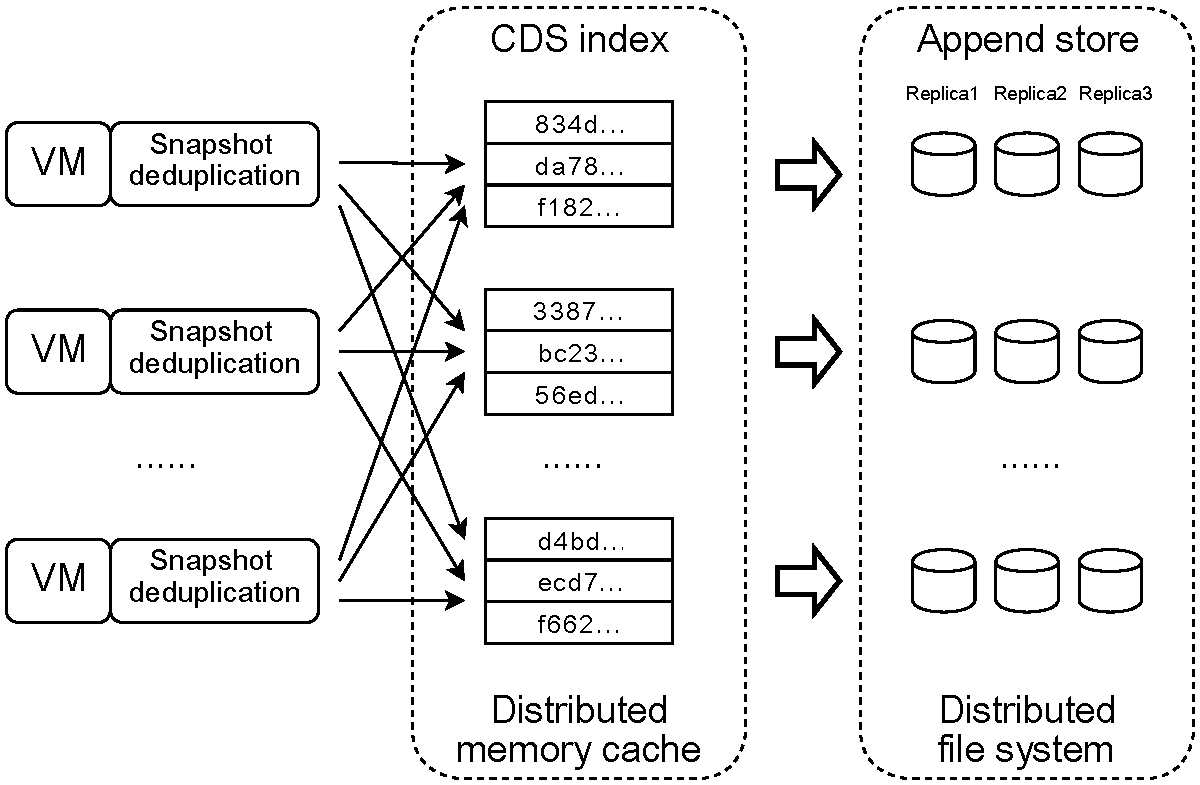
\includegraphics[width=6in]{images/socc_arch_cluster}
    \caption{System Architecture}
    \label{fig:arch_vm}
\end{figure*}

\subsection{A VM-centric snapshot store for backup data}
\label{sect:store}
We build the snapshot storage on the top of a distributed file system.
Following the VM-centric idea for the purpose of fault isolation,
each VM has its own snapshot store, containing new data chunks which are considered
to be non-duplicates.
There is also a special store containing all PDS chunks shared among different VMs.
As shown in Fig.\ref{fig:as_arch}, we explain the data structure of snapshot stores as follows.

\begin{itemize}
\item Data of each VM snapshot store excluding PDS is divided into a set of containers and 
each container is approximately 1GB. 
The reason for dividing the snapshot into containers is to simplify the compaction process
conducted periodically. As discussed later, data chunks are deleted from old snapshots
and chunks without any reference from other snapshots can be removed by this compaction process.
By limiting the size of a container, we can effectively control the length of each compaction process.
The compaction  routine can work on one container at a time and copy used data chunks to another container. 

Each container is further divided into a set of chunk data groups. Each chunk group is composed of
a set of data chunks and is the basic unit in data access and retrieval. 
In writing a chunk during backup, the system accumulates data chunks and store the entire
group as a unit after a compression.
When accessing a particular chunk, its chunk group is retrieved from the storage
and uncompressed. Given the high spatial locality and usefulness of prefetching  in 
snapshot chunk accessing~\cite{Guo2011,foundation08},
retrieval of  a data chunk  group naturally works well with prefetching. 
A  typical chunk group contains 100 to 1000 chunks, with an average size of 
200-600 chunks.

\item Each data container is represented by three files in the DFS:
1) the container data file holds the actual content, 
2) the container index file is responsible for translating a data reference
into its location within a container, and 
3) a chunk deletion log file records all the deletion requests within  the container.

\item A data chunk reference stored in the index of snapshot recipes
is composed of two parts: a container ID with 2 bytes and a local chunk ID with 6 bytes.
Each container maintains a local  chunk counter and assigns the current number 
as a chunk ID  when  a new chunk is added to this  container. 
Since data chunks are always appended to a snapshot store during backup, 
a local chunk ID is monotonically increasing.
When a snapshot chunk is to be accessed, the recipe for the snapshot will point a data chunk
in the PDS store or in a non-PDS VM snapshot  store. 
Using  a container ID, the corresponding container index file of this VM is accessed and 
the chunk group is identified using a simple chunk ID range search. Once the chunk group is loaded to memory, 
its header contains the exact offset of the corresponding chunk ID and the content is then accessed from the memory buffer.

\item The PDS chunks are a set of commonly used data and they are stored in one PDS file.
Since the total file size is relatively small, and
PDS data is re-calculated periodically, the PDS data file and its index are rebuilt completely. 
Each reference to a PDS data chunk in the PDS index is the offset within the PDS file, and the chunk size.

\end{itemize}

\begin{figure}[htbp]
  \centering
  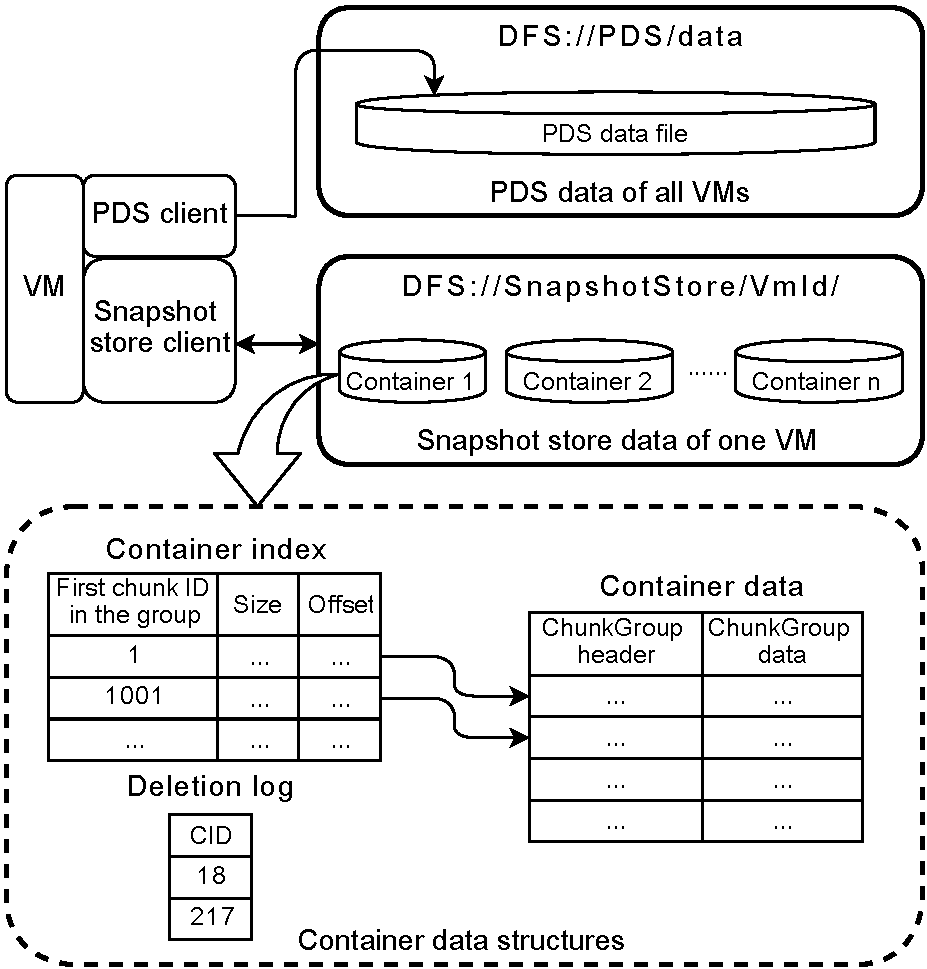
\epsfig{file=images/sstore_arch, width=3in}
  \caption{Data structure of a VM snapshot store.}
  \label{fig:as_arch}
\end{figure}

A snapshot  store supports three API calls.
\begin{itemize}
\item {\em Put(data)}. This places data chunk into the snapshot store and returns a reference to be stored in 
the recipe metadata of a snapshot. 
The write requests to append data chunks to a VM store are accumulated at the client side. 
When the number of write requests reaches a fixed group size, the snapshot store client compresses
the accumulated   chunk group, adds a chunk group index  to the beginning of the group, and then
appends the header and data  to the corresponding VM file.
A new container  index entry is also created for each chunk group and is written the corresponding
container index file.
The writing of PDS data chunks is conducted periodically when there is a new PDS calculation.
\item{\em Get(reference)}.
The fetch operation for the PDS data chunk is straightforward since each reference contains 
the offset and size within the PDS  underlying  file.
We also maintain a small data cache for the PDS data service to speedup common data fetching.

To read a non-PDS chunk using its reference with container ID and local chunk ID,  the snapshot store client first loads the
corresponding VM's container index file specified by the container ID, then searches the chunk
groups  using their  chunk ID coverage.
After that, it reads the identified chunk group from DFS, decompresses it, and seeks to the exact chunk data 
specified by the chunk ID. 
Finally, the client updates its internal chunk data cache with the newly loaded content to 
anticipate future sequential reads.
\item {\em Delete(reference)}.
Chunk deletion occurs when a snapshot expires or gets deleted explicitly by a user
and we will discuss the snapshot deletion in detail in the following subsection.
When deletion requests are issued for a specific container,
those requests are simply recorded into the  container's deletion log initially and thus  a lazy
deletion strategy is exercised.
Once local chunk IDs appear in
the deletion log, they will not be referenced by any future snapshot and can be safely deleted when needed. 
Periodically, the snapshot  store picks those containers with an excessive
number of deletion requests to  compact and  reclaim the corresponding disk space. 
During compaction, the snapshot store creates a new container (with the same container ID) to replace the 
existing one. This is done by sequentially scanning the old container, copying all the chunks that are not 
found in the deletion log to the new container, and creating new chunk groups and indices. 
Every local chunk ID however is directly copied rather than re-generated. This
process leaves holes in the CID values, but preserves the sorted order.
As a result, all data references stored 
in upper level recipes are permanent and stable, and the data reading process
is as efficient as before. Maintaining the stability of chunk IDs also ensures that recipes do not
depend directly on physical storage locations.
\end{itemize}

\subsection{ VM-centric Approximate Snapshot Deletion with Leak Repair}
\label{sect:delete}

\begin{figure}[htbp]
  \centering
  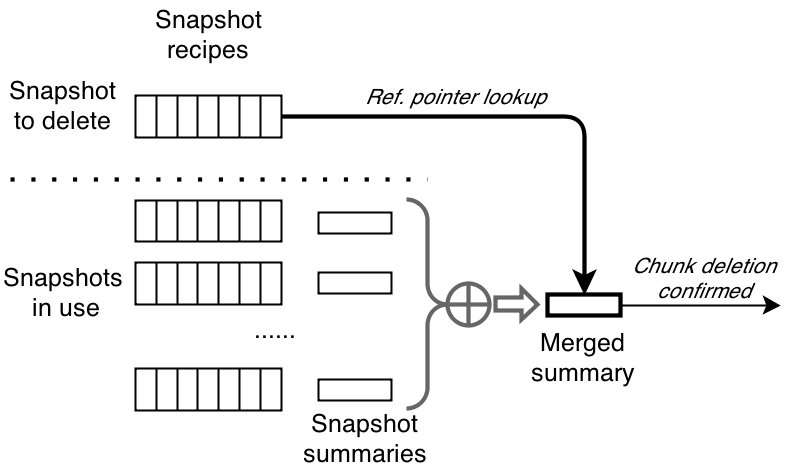
\epsfig{file=images/deletion.png, width=3.5in}
  \caption{Approximate deletion}
  \label{fig:deletion_flow}
\end{figure}

In a busy VM cluster, snapshot deletions can occur frequently.
Deduplication complicates the deletion process because space saving relies on the sharing of data
and it requires the global reference of deleted chunks to be identified before  they can be safely removed.
While we can use the mark-and-sweep technique~\cite{Guo2011}, 
it still takes significant resource to conduct this process every time there is a snapshot deletion.
In the case of Alibaba, snapshot backup is conducted automatically and there are 
about 10 snapshot stored for every user. When there is
a new snapshot created every day,  there will be  a snapshot expired everyday to maintain
a balanced storage use. 

We seek a fast solution with a low resource usage to delete snapshots.
Our VM-centric snapshot storage design simplifies the deletion process since 
we can focus on  unreferenced chunks within each VM.
The PDS data chunks are commonly shared all VMs and we do not consider them
during snapshot deletion.  The selection of PDS data chunks is updated periodically independent of snapshot deletion process.
Another resource-saving strategy we propose is
an {\em approximate} deletion strategy to trade deletion accuracy for
speed and resource usage. Our method sacrifices a small percent of storage leakage
to efficiently identify unused chunks.

The algorithm contains three aspects.

\begin{itemize}
\item {\bf Computation for snapshot fingerprint summary.}
Every time there is a new snapshot created,
we compute a Bloom-filter with $z$ bits as the summary of reference pointers for all non-PDS chunks used 
in this snapshot. Given $h$ snapshots stored for a VM, there are $h$ summary vectors maintained.

\item {\bf Approximate deletion with fast summary comparison.}
When there is a snapshot deletion,  
we need to identify if  chunks to be deleted from that snapshot
are still used by other snapshots. 
This is done approximately and quickly by comparing the 
reference pointers of deleted snapshot with
the merged reference Bloom-filter summary of other live snapshots.
The merging of live snapshot Bloom-filter bits uses the logical OR operator 
and the merged vector still takes $z$ bits.
Since the number of live snapshots $h$ is limited for
each VM, 
the time and memory cost of this comparison is small, linear to the number of chunks to be deleted.

If a chunk's reference pointer is not found in the merged summary vector, we are sure that
this chunk is not used by any live snapshots, thus it's safe delete it. 
However, among all the chunks to be deleted, 
there is a small percentage of unused chunks  which
are misjudged as  being in use, resulting in a storage leakage.

\item {\bf Periodic repair of leakage}.
%[exlpain why second Bloom filter, why scan append store]
Leakage repair is conducted periodically to fix the above approximation error.
This procedure compares the live chunks for each VM with what are truly used through the VM snapshot metadata recipe.
That requires a scanning of all chunks in a VM; however it is a VM-specific procedure and thus
the cost is relatively small compared to the traditional mark-sweep procedure~\cite{Guo2011} which scans snapshot 
chunks from all VMs.
For example,
consider each reference pointer consumes 8 bytes plus  1 mark bit, a VM that has 40GB backup data with about
10 million chunks will need less than 90MB of memory to complete a VM-specific mark-sweep process.
\end{itemize}

%{\bf Discussion}
We now estimate the size of storage leakage and how often leak repair needs to be conducted,
given  a VM which keeps $h$ snapshots in the backup storage, and it creates and deletes one snapshot
everyday. Let $u$ be the total number of chunks brought by the initial backup, $\Delta u$ be the average
number of additional unique chunks added from one snapshot to the next snapshot version. Then the total number of unique
chunks used in a VM is about:
\[
U = u + (h-1)\Delta u.
\]

Each Bloom filter vector has  $z$ bits for each snapshot and let $j$ be the number of hash functions used by the
Bloom filter. The probablity that a particular bit is 0  in all $h$ summary vectors is  
$(1- \frac{1}{z}) ^{j U}$. Notice that a chunk may appear multiple times in these summary vectors; however, this should not 
increase the probability of being a 0 bit in all $h$ summary vectors.
Then the misjudgment rate of being in use $\epsilon$ is: 
\begin{equation}
\label{eq:falserate}
\epsilon = (1-(1-\frac{1}{z})^{jU})^j.
\end{equation}


For each snapshot deletion, the amount of chunks need to be deleted is nearly identical to the number of
newly add chunks $\Delta u$. 
Let $R$ be the total number of runs of approximate deletion between two consecutive 
repairs. we estimate  the total leakage $L$ after $R$ runs as:
\[
L = R \Delta u \epsilon
\]

When leakage ratio $L/U$ exceeds a pre-defined threshold $\tau$, we need to execute a leak repair:

\begin{equation}
\label{eq:leakrepair}
\frac{L}{U} = \frac{R \Delta u \epsilon}{u+(h-1)\Delta u } > \tau 
\Longrightarrow R > \frac{\tau}{\epsilon}\times\frac{u + (h-1)\Delta u}{\Delta u}
\end{equation}

For example in our tested dataset,  
each VM keeps $h=10$ snapshots and each snapshot has
about 1-5\% of new data. Thus $\frac{\Delta u}{u} \leq 0.05$. For a 40GB snapshot, $u\approx  10$ millions.
Then $U=10.45$ millions.
We choose  $\epsilon = 0.01$ and $\tau=0.1$.  From Equation~\ref{eq:falserate}, 
$z=10U=100.45$ million bits. From Equation~\ref{eq:leakrepair}, 
leak repair should be triggered once for every R=290 runs of approximate deletion. 
When one machine hosts 25 VMs and there is one snapshot deletion per day per VM, there would be 
only one full leak repair for one VM scheduled for every 12 days. Each repairs uses at most  90MB memory on average
as discussed earlier and takes a short period of time.


\section{Evaluation}
\label{sect:evaluation}
We have implemented and evaluated a prototype of our VC scheme on a Linux cluster of machines with
8-core 3.1Ghz AMD FX-8120 and 16 GB RAM. 
Our implementation is based on Alibaba cloud platform~\cite{Aliyun,WeiZhangIEEE}
and the underlying DFS uses  QFS with default replication degree 3 while the PDS replication degree is 6.
Our evaluation objective is to
study the benefit in fault tolerance and   deduplication efficiency of VC and compare it
with an alternative VO design. We also and assess backup throughput and  resource usage for a large number of VMs.

We will compare VC with a VO approach  using stateless routing with binning (SRB) 
based on~\cite{Dong2011,extreme_binning09}.
SRB executes a distributed deduplication by routing a data chunk to one of cluster machines~\cite{Dong2011}
using  a min-hash function discussed in \cite{extreme_binning09}. Once a data chunk is routed to
a machine, this chunk is compared with the fingerprint index within this machine locally. 

\subsection{Settings}
We have performed a trace-driven study using a production dataset~\cite{WeiZhangIEEE} from 
Alibaba Aliyun's cloud platform with about 100 machines. 
Each machine hosts upto 25 VMs and each VM keeps 10 automatically-generated snapshots in the storage system while
a user may instruct extra snapshots to be saved.
The VMs of the sampled data set use popular operating systems such as 
Debian, Ubuntu, Redhat, CentOS, win2008 and win2003. 
The backup of VM snapshots is required to complete within few  hours every night.
Based on our study of production  data,  each VM has about 40GB of storage  data  on average
including OS and user data disk.
%All data are divided into 2 MB fix-sized segments and 
The signature for variable-sized blocks is computed using their SHA-1 hash~\cite{similar94,rabin81}. 
%Each segment is divided into 
%variable-sized content chunks with an average size of 4KB.
%Popularity of data blocks are collected through global counting and 
%and top popular ones ($\delta=2\%$)  are  kept in the PDS, as discussed in Section~\ref{sect:store}.

\subsection{Impact on Fault Isolation}

 Table~\ref{tab:vm-availability} shows the availability of VM snapshots when 
there are up to 20 machine nodes failed in a 100-node cluster and  a 1000-node cluster. 
%Two VC curves use $V_c=1250$ and $V_c=2500$ representing the average number of VMs that share a PDS file system block. 
We assume that every VM points to every filesystem block in the PDS ($V_c=p*V$), which is to be expected when PDS
blocks are sorted by hash, as their order is randomized.
%$V_c=2500$ represents  the absolute worst case for 2500 VMs. 
%The VO curve has  $V_o=6.3$ which is the average number of VMs that share a file system block in our smaller dataset.
%To get this number, we perform perfect deduplication over 105 VMs, append unique chunks to a DFS file and
%count the number of dependencies from a file system block to VM.
%In the scenario of having 2500 VMs, this number can only increase, thus this number represents the best
%case for VO approach. 
%Our results show that the VC approach even with $V_c=2500$ has a higher availability than VO.
%For example, with 10 machines failed, VO with 98.5\% availability would lose snapshots of 37 VMs 
%while VC with 99.9\% loses snapshots of 2.5 VMs.
%The key reason is that  $N_1 +N_2 < N_o$, caused by the fact that the VM-centric approach localizes deduplication
%and packs  data blocks for one VM as much as possible.  The extra replication
%for PDS blocks also significantly increases the snapshot availability even when
%a PDS file block is shared by every VM.
%=======
%Figure~\ref{tab:vm-availability} shows the availability of VM snapshots
%as storage nodes fail. 
%We assume a random distirbution of 64MB filesystem
%blocks (FSBs). where FSBs are not randomly distributed availability might
%be improved by limiting the number of storage nodes a particualr VM depends
%on but we take the conservative approach. We compare VO, the expected case for
%VC ($V_c=p*V/2$), and the worst case for VC ($V_c=p*V/2$). We set $V_o=6.3$
%based on measured values in our dataset.
To obtain VO sharing of file blocks, we perform perfect deduplication over 105 VMs, 
append unique chunks to a DFS file and
count the number of dependencies from a file system block to VM.
%In the case of having 2500 or even 25000 VMs, this number can only increase, thus this number represents the best
%case for VO approach. 
Our results show that even the worst case for VC (where $v_c=p*V$) has a higher availability than VO.
%Our VM-centric approach shows significant improvements
%in VM availability.
For example, with 5/100 machines failed and 25 VMs per machine, VO with 93.256\% availability would lose data in 169 VMs 
while VC with 97.763\% loses data for 56 VMs.
The key reason is that for most data in VC, only a single
VM can be affected by the loss of a single FSB. Since most FSBs contain blocks for a single VM, VMs can point to a smaller number of FSBs.
% because our VM-centric approach
%localizes deduplication.  

Although the loss of a PDS block affects many VMs,
by increasing replication for those blocks we minimize the affect on VM availability.
%By having extra replicas for the PDS data, we reduce the failure rate of PDS
%FSBs enough that the failure rate for the VM approaches the failure rate of the
%Non-PDS blocks. This minimizes the drop in availability between the expected
%and worst case for VC.
%
%One of the advantages of VC is that there is a division between
%popular and non-popular data to facilitate improved reliability. 
Figure~\ref{fig:pds-replication}) shows
the impact of  to increasing PDS data replication. 
While the impact on replication storage cost is small, 
the replication degree 6  has a significant improvement over 4, but  the availability is about
the same for $r_c=6$ and $r_c=9$.
 
%This is because, as described before, the availability of the VM approaches the
%availiability of the Non-PDS data as the failure rate of PDS data gets very small.

\comments{
\begin{figure}[ht]
    \centering
    \begin{subfigure}%{.5\textwidth}
      \centering
      %\includegraphics[scale=.45,natwidth=511,natheight=276]{vo_links}
            \begin{tikzpicture}
                    \begin{axis}[
                    tick label style={font=\scriptsize},
                    tick style=thin,
                    width=0.5\linewidth,
                    title={\small $p=100$},
                    cycle list={
                        {blue,thin,solid,mark=none},
                        {red,thin,densely dashed,mark=none},
                        {red,thin,densely dotted,mark=none}
                    },
                    xlabel={\tiny Failed nodes},
                    ylabel={\tiny VM Availability (\%)},
                    %extra y ticks={99.9}, %if important numbers are missing
                    mark options=solid,
                    legend columns=-1,
                    legend style={
                        font=\small\sffamily,
                        cells={anchor=west}, %legend entry alignment
                        legend pos=south west %legend position
                    },
                    legend to name=legend:vm-availability,
                    %reverse legend,
                    ]
                    \addplot table[x=NodesFailed,y=VO]{figures/node_failures_100.txt};
                    \addlegendentry{VO}
                    \addplot table[x=NodesFailed,y=VC3]{figures/node_failures_100.txt};
                    \addlegendentry{VC}
                    %\addplot table[x=NodesFailed,y=VCOpt1]{figures/node_failures_100.txt};
                    %\addlegendentry{VC (CDS ordering)}
                    \end{axis}
            \end{tikzpicture}
      %\caption{100 machine cluster.}
      \label{fig:vm-availability-100}
    \end{subfigure}%
    \begin{subfigure}%{.5\textwidth}
  \centering
  %\includegraphics[scale=.45,natwidth=511,natheight=276]{vo_links}
	\begin{tikzpicture}
            %the expressions in this plot are simply to trick pgfplots into not expanding the y range, and don't actually change the data
            % expression used: (99.999+((y-99.999)*1000)/1000)
            \pgfplotsset{/pgf/number format/.cd,
                fixed,precision=4}
		\begin{axis}[
                    width=0.5\linewidth,
                    tick label style={font=\scriptsize},
                    tick style=thin,
		title={\small $p=1000$},
                %ymin=099.9991,
                %ymax=100.0002,
                %ytick=data,
                %yticklabels from table={figures/vm_availability_1000.txt}{[index]1},
                yticklabel={%this is a hack to get around the small yrange
                    \pgfmathfloatparse{99.999+\tick/1000}
                    \pgfmathprintnumber{\pgfmathresult}
                },
                cycle list={
                    {blue,thin,solid,mark=none},
                    {red,thin,densely dashed,mark=none},
                    {red,thin,densely dotted,mark=none}
                },
		xlabel={\tiny Failed nodes},
		ylabel={\tiny VM Availability (\%)},
		%extra y ticks={99.99}, %if important numbers are missing
                mark options=solid,
                legend style={
                    cells={anchor=west}, %legend entry alignment
                    legend pos=south west %legend position
                },
                %reverse legend,
		]
                %\addplot table[x=NodesFailed,y=VO1]{figures/vm_availability_1000.txt};
                \addplot table[x=NodesFailed,y expr=(\thisrow{VO}-99.999)*1000]{figures/node_failures_1000.txt};
                %\addlegendentry{$VO\,6.3$ (optimistic)}
                %\addplot table[x=NodesFailed,y=VC1]{figures/vm_availability_1000.txt};
                \addplot table[x=NodesFailed,y expr=(\thisrow{VC3}-99.999)*1000]{figures/node_failures_1000.txt};
                %\addlegendentry{$VC\,1250$ (estimated)}
                %\addplot table[x=NodesFailed,y=VC2]{figures/vm_availability_1000.txt};
                \addplot table[x=NodesFailed,y expr=(\thisrow{VCWC1}-99.999)*1000]{figures/node_failures_1000.txt};
                %\addlegendentry{$VC\,2500000$ (worst-case)}
                %\addplot table[x=NodesFailed,y=VO2]{figures/vm_availability.txt};
                %\addlegendentry{$VO\,20$ (optimistic)}
		\end{axis}
	\end{tikzpicture}
        %\caption{1000 machine cluster.}
  \label{fig:vm-availability-1000}
\end{subfigure}
    \pgfplotslegendfromname{legend:vm-availability}
      \caption{Availability of VM snapshots for VO and VC when failed machines vary
from 1 to 40.  Non-PDS replication is fixed
at 3 and PDS replication is 6 \emph{THIS PLOT IS BEING REPLACED BY A TABLE} 
      }
      \label{fig:vm-availability}
   
 
\end{figure}
}
\begin{table}
  \centering
    \footnotesize
    \tabcolsep=0.11cm
    \pgfplotstabletypeset[
        columns={NodesFailed,VO100,VC100,VO1000,VC1000},
        columns/NodesFailed/.style={
            column name={\multirow{3}{*}{Failures ($d$)}}
        },
        columns/VO100/.style={
            column name={
                \multicolumn{4}{c|}{VM Availability(\%)}\\&
                \multicolumn{2}{c|}{$p=100$}&\multicolumn{2}{c|}{$p=1000$}\\&
            VO},
            fixed, precision=6
        },
        columns/VC100/.style={
            column name={VC},
            fixed, precision=6},
        columns/VO1000/.style={
            column name={VO},
            fixed, precision=6},
        columns/VC1000/.style={
            column name={VC},
            fixed, precision=6},
        every head row/.style={
            before row={\hline},
            after row={\hline},
        },
        every last row/.style={after row=\hline},
        column type/.add={}{|},
        every first column/.style={column type/.add={|}{}},
        %the below rows can be used to extract rows 3,5,10,20 from rows 0-40
        %skip rows between index={0}{3},
        %skip rows between index={4}{5},
        %skip rows between index={6}{10},
        %skip rows between index={11}{20},
        %skip rows between index={21}{41}
    ]{figures/availability_table.txt}
    \caption{Availability of VM snapshots for VO and VC.}
    \label{tab:vm-availability}
\end{table}


\begin{figure}[htbp]
  \centering
	\begin{tikzpicture}
		\begin{axis}[
                        width=\linewidth,
                        height=0.6\linewidth,
		%title={PDS Replication affect on availability},
		xlabel={Failed storage nodes},
		ylabel={VM Snapshot Availability (\%)},
                xmin=0,
                xmax=20,
		%extra y ticks={99.9}, %if important numbers are missing
                mark options=solid,
                legend style={
                    cells={anchor=west}, %legend entry alignment
                    legend pos=south west %legend position
                },
                reverse legend,
		]
                \addplot table[x=NodesFailed,y=VC1]{figures/node_failures_100.txt};
                \addplot table[x=NodesFailed,y=VC2]{figures/node_failures_100.txt};
                \addplot table[x=NodesFailed,y=VC3]{figures/node_failures_100.txt};
                \addplot table[x=NodesFailed,y=VC4]{figures/node_failures_100.txt};
                \legend{$r_c=4$,$r_c=5$,$r_c=6$, $r_c=9$}
		\end{axis}
	\end{tikzpicture}
  \caption{Availability of VM snapshots in VC with different PDS replication degrees}
  \label{fig:pds-replication}
\end{figure}

\subsection{Deduplication Efficiency}
%this version combines the old and the minhash alg. to compare against srb
\begin{figure}[ht]
  \centering
    \begin{tikzpicture}
            \begin{axis}[
            %title={Ex-Binning Efficiency},
            width=\linewidth,
            height=0.75\linewidth,
            cycle list={%
                {blue,solid,mark=square*},
                {blue,solid,mark=triangle*,mark size=1.5},
                {blue,solid,mark=diamond*,mark size=1.5},
                %{blue,solid,mark=pentagon*,mark size=1.4},
                {red,draw=red,densely dotted,mark=square},
                %{red,densely dotted,mark=triangle,mark size=1.5},
                %{red,densely dotted,mark=diamond,mark size=1.5},
                {brown,densely dashed,mark=*},
                %{red,densely dotted,mark=o},
                %{red,densely dotted,mark=pentagon,mark size=1.4},
            },
            mark repeat={10},
            xlabel={Number of VMs added},
            ylabel={Dedup. Efficiency (\%)},
            xmin=0,
            ymin=85,
            ymax=100,
            %extra y ticks={4.5,5.5,6.5} %to add extra ticks
            mark options=solid,
            legend pos=south west,
            legend columns=2,
            legend style={
                font={\tiny\sffamily},
                %at={(0.5,-0.2)},
                %anchor=north
            },
            ]
            \addplot table[x=VMs,y=MHcds4] {figures/exbin_efficiency_comparison2.txt};
            \addplot table[x=VMs,y=MHcds2] {figures/exbin_efficiency_comparison2.txt};
            %\addplot table[x=VMs,y=MHcds1] {figures/exbin_efficiency_comparison2.txt};
            \addplot table[x=VMs,y=MHNocds] {figures/exbin_efficiency_comparison2.txt};
            %\addplot table[x=VMs,y=cds4] {figures/exbin_efficiency_comparison2.txt};
            \addplot table[x=VMs,y=cds2] {figures/exbin_efficiency_comparison2.txt};
            %\addplot table[x=VMs,y=cds1] {figures/exbin_efficiency_comparison2.txt};
            \addplot table[x=VMs,y=exbin] {figures/exbin_efficiency_comparison2.txt};
            \legend{VC( $\sigma=4\%$),
                VC($\sigma=2\%$),
                %VC MH($\sigma=1\%$),
                VC(No PDS),
                %VC($\sigma=4\%$),
                VC(No MH\,$\sigma=2\%$),
                %VC($\sigma=1\%$),
                SRB
            };
            \end{axis}
    \end{tikzpicture}
    \caption{Deduplication efficiency of VC and SRB.}
  \label{fig:exbin-efficiency-graph2}
\end{figure}

Figure~\ref{fig:exbin-efficiency-graph2} shows the deduplication efficiency for SRB and VC.
% <<<<<<< HEAD
% Our deduplication efficiency is defined as the percent of duplicate chunks
% which are detected and deduplicated, so only global perfect deduplication can have 100\% efficiency.
% The figure also compares several PDS sizes chosen for VC. ``$\sigma=2\%$'' 
% is defined in Table~\ref{tab:symbol}. 
% =======
Deduplication efficiency is defined as the percent of duplicate chunks
which are detected and deduplicated, so only global perfect deduplication can have 100\% efficiency.
 We also compare several PDS sizes chosen for VC.
%(see Table~\ref{tab:symbol} for definition of ``$\sigma=2\%$'')
%we allocate the space of distributed shared memory  to accommodate 2\%
%of data chunks shared among VMs, as defined in 
With $\sigma=2\%$, memory usage for PDS index lookup per machine is about 100MB per machine
and  the deduplication efficiency can reach 96.489\%.
When $\sigma=4\%$, the deduplication efficiency can reach 97.027\% while space consumption increases to 200MB per machine. 
The loss of efficiency in VC is caused by the restriction of the physical memory available
in the cluster to support fast in-memory PDS index lookup. 
%In the extreme case if we put all the fingerprint into PDS 
%index ($\sigma=100\%$) then VC will have 100\% efficiency.
SRB can deliver up to 97.935\% deduplication efficiency which is slightly better than VC.
Thus this represents a tradeoff: VC provides better fault tolerance and fast
approximate deletion with a competitive (but slightly lower) deduplication
efficiency.
%its loss of efficiency is caused by the routing of data chunks which restricts the search scope
%of duplicate detection.
%SRB provides slightly better deduplication efficiency than our VC approach, which we accept
%because we are rewarded by architecture-wise benefits such as fault-tolerance and fast 
%Though not our primary goal, this result does show that VC can remove a competitive amount of duplicates.

Figure~\ref{fig:exbin-efficiency-graph2} also shows the effectiveness of the local similarity-based search in VC.
Without this (i.e. when we only check the parent segment at the same offset), when an entire
segment is moved to another location on disk, for example when a file is rewritten
rather than modified in place, the deduplication opportunity is missed. We have found that in
approximately 1/3 of the VMs in our dataset this movement happens frequently,
so the similarity search becomes important for those VMs.
In general, our experiments show that
dirty-bit detection at the segment level can reduce the data size to about 24\% of original data, 
which leads  about 76\% reduction.
Similarity-guided local search can further reduce the data size
to about 12\% of original size, namely it delivers additional 12\% reduction.
The PDS-based cross-VM detection with $\sigma=2\% $
can reduce the  size further to 5.6\% of original size, namely it 
delivers additional 6.4\% reduction.

%Figure~\ref{fig:exbin-efficiency-graph2} also shows the benefits of our minhash
%similar segment search in the parent snapshot. 

\subsection{Resource Usage and Processing Time}

\comments{
\begin{table}
    \begin{tabular}{|c|c|}
    \hline
    PDS replication degree & Disk usage per machine  \\ \hline
    3                      & 3065GB             \\ \hline
    4                      & 3072GB             \\ \hline
    5                      & 3079GB             \\ \hline
    6                      & 3086GB             \\ \hline
    7                      & 3093GB             \\ \hline
    \end{tabular}
\caption{Storage space cost per machine for DFS under different PDS replication degree}
\label{tab:replication_cost}
\end{table}
}

{\bf Storage cost of replication.} 
%Table ~\ref{tab:replication_cost} shows the total storage space required by 
%VC as the PDS replication degree changes while non-PDS replication degree is fixed as 3. 
The total storage  for all VM snapshots in each physical machine takes about 3.065TB on average when
the replication degree of both PDS and non-PDS data is 3. 
Allocating  one extra  copy for PDS data only adds  7GB in total per machine.
Thus PDS replication degree 6 only adds the total space by 0.685\% while PDS replication degree 9 adds 1.37\% 
space overhead, which is still small.
%The increase in storage cost is minimal because the PDS makes up a 
%small percent of the total storage space, while increasing replication degree has a  more significant benefit for
%availability as shown in Figure~\ref{fig:pds-replication}.

\begin{table}
    \begin{tabular}{|c|c|c|c|c|c|}
    \hline
    Tasks & CPU & Mem &Read &  Write  & Time  \\ 
    & & (MB)          &(MB/s) &  (MB/s) & (hrs) \\ \hline
%    1     & 19\% & 118.1 & 50MB/s 8.37 & 1.314\\ \hline
    1     & 19\% & 118 & 50 & 8.4 & 1.31\\ \hline
%    2     & 35\% & 131.8 & 9.0 & 1.226\\ \hline
    2     & 35\% & 132 &50  & 9.0 & 1.23\\ \hline
    %4     & 63\% & 154.1 & 9.3 & 1.179\\ \hline
    4     & 63\% & 154&50   & 9.3 & 1.18\\ \hline
%    6     & 77\% & 171.9 & 9.46 & 1.162\\ \hline
%    8     & 82\% & 90.5 & 89.2 & \\ \hline
%    10                      & 85\% & 97.2   & 90.4 \\ \hline
%    12                      & 91\% & 95.6    & 91.5 \\ \hline
    \end{tabular}
\caption{Resource usage of concurrent backup tasks at each machine}
\label{tab:resource_usage}
\end{table}

{\bf Memory and disk bandwidth usage with multi-VM processing}. 
We have further studied the memory and disk bandwidth usage 
when running concurrent VM snapshot backup on each machine with $\delta=2\%$. 
Table ~\ref{tab:resource_usage} gives the resource usage  when
running 1 or multiple  VM backup tasks at the same time on each physical machine. 
``CPU'' column is the percentage of a core usage. 
``Mem'' column includes 100MB memory usage for PDS index and other space cost for executing deduplication tasks such as 
receipt metadata and cache. 
``Read'' column is controlled as 50MB/s bandwidth usage so that other cloud services are not impacted a lot.
``Write'' column is the I/O write usage of QFS and notice that each QFS write leads writes in multiple machines due to
data replication.     
% [ NOT REASONABLE: Notice that memory and CPU used by PDS index and QFS are not included since they belong to 
% the cloud infrastructure services and are shared among many applications.]
%We see our hybrid deduplication scheme only occupies a small amount of system resources. 
%The  local deduplication only needs to keep the parent snapshot recipe and a few similar segment recipes in 
%memory during duplicate detection.

Table ~\ref{tab:resource_usage} shows that  a single backup task per node can complete the backup of the entire
VM cluster in about 1.58 hours. Since there are about 25 VMs per machine, we could execute
more tasks in parallel at each machine. But adding more backup concurrency does not shorten the overall time
a lot because of the controlled  disk read time.
%,  we can still process raw data at near 175 MB/s. If we consider the extreme case in which each machine has 25 VMs
%at 40GB size, our snapshot system can finish backing up all the VMs (1TB total) in 1.58 hours.

{\bf Processing Time breakdown}.
Figure~\ref{fig:vc_srb_combined} shows
the  average  processing  time of  a VM segment under VC and SRB. 
VC uses $\sigma=2\%$ and $4\%$.
It has a breakdown of time for reading data, updating the metadata, network latency to visit
a remote machine, and index access for fingerprint comparison.
The change of $\sigma$ does not significantly affect the overall backup speed as
PDS lookup takes only a small amount of time.
SRB has a higher index access and fingerprint comparison because once a chunk is routed to a machine,
it relies on this local machine to access its index (often on the disk, supported by a Bloom filter) 
and perform comparison.
VC is faster for index access because it conducts in-memory local search first and then
accesses  the PDS on distributed shared memory.  
SRB spends  slighter more time in  reading data and updates because it also updates the on-disk
local meta data index.
Overall,  VC is faster than SRB, though data reading dominates the processing time for both algorithms.
%Figure~\ref{fig:vc_srb_combined} also reports the average backup time for a VM in VC when
%varying the PDS size.  It lists the time distribution for data reading,
%similarity-guided local search, cross-VM PDS lookup, and non-duplicate data writing. 
%While data reading dominates the backup process, PDS lookup spends about a similar amount
%of time as local search.

\begin{figure}[htbp]
  \centering
  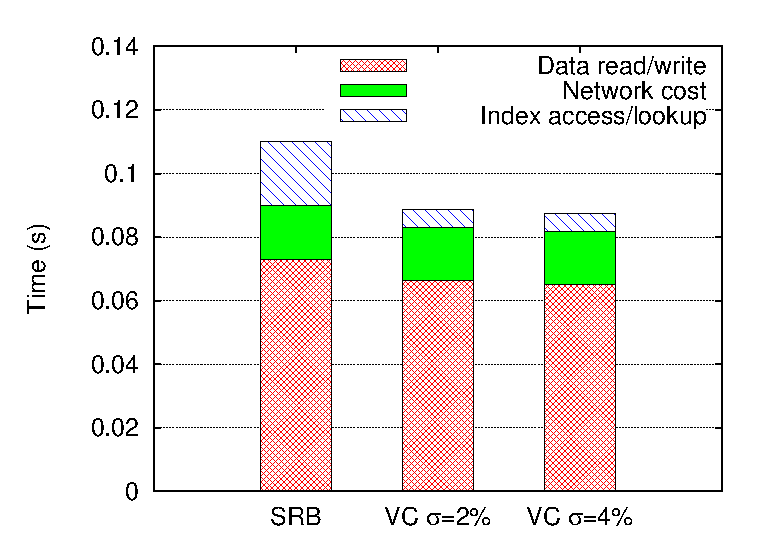
\epsfig{file=figures/vc_srb_combined, width=3in}
  \caption{Average time to backup a dirty VM segment under SRB and VC}
  \label{fig:vc_srb_combined}
\end{figure}

% \begin{figure}[htbp]
%   \centering
%   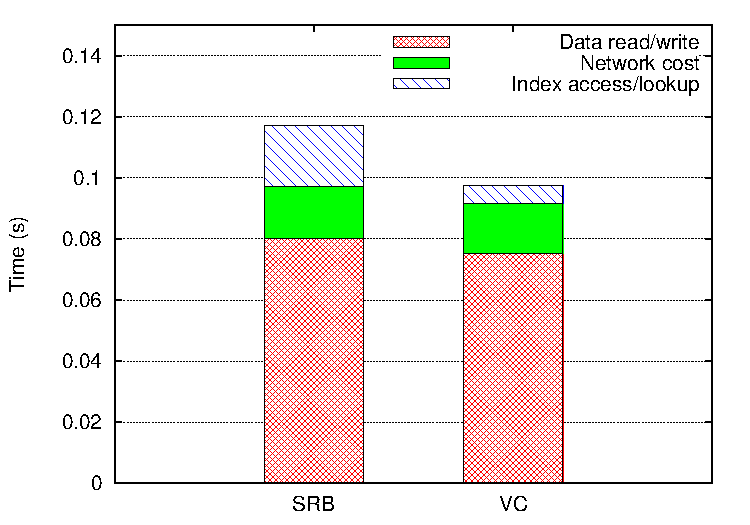
\epsfig{file=figures/srb_vs_vc, width=3in}
%   \caption{Time to backup a dirty VM segment under SRB and VC}
%   \label{fig:srb_vs_vc}
% \end{figure}


% \begin{figure}
%     \centering
%     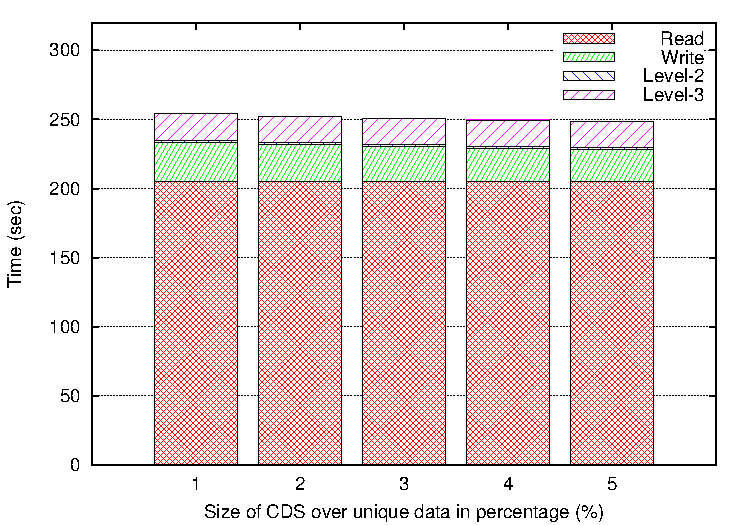
\includegraphics[width=3in]{figures/single_backup_time}
%     \caption{Average time to backup a VM in VC with varying PDS sizes}
%     \label{fig:single_vm_backup}
% \end{figure}


\begin{table*}[t]
    \centering
    \begin{tabular}{c|ccc|ccc}
    Num. of concurrent      & \multicolumn{3}{c|}{Throughput without}    & \multicolumn{3}{c}{Throughput with} \\
    backup tasks            & \multicolumn{3}{c|}{I/O throttling (MB/s)} & \multicolumn{3}{c}{I/O throttling (MB/s)} \\ \cline{2-7}
    per node                & Raw                                        & Snapshot Store & QFS  & Raw                                    & Snapshot Store & QFS  \\ \hline
    1                       & 1369.6                                     & 148.0          & 18.0 & 171.3                                  & 18.5           & 2.26 \\
    2                       & 2408.5                                     & 260.2          & 31.7 & 201.3                                  & 21.8           & 2.66 \\
    4                       & 4101.8                                     & 443.3          & 54.1 & 217.8                                  & 23.5           & 2.87 \\
    6                       & 5456.5                                     & 589.7          & 72.0 & 224.1                                  & 24.2           & 2.96 \\
    \end{tabular}
\caption{Throughput of software layers under different concurrency}
\label{tab:throughput}
\end{table*}
{\bf Throughput of software layers.}
Table~\ref{tab:throughput} shows the  average throughput of software layer
when I/O is throttled under 50MB/second and when there is no restriction.
%machine when all machine nodes execute one or multiple MV backup tasks.
``Raw'' column is the throughput  of the backup service  per machine.
``Snapshot store" is the  write throughput of the snapshot store layer and the gap between this
column and  ``Raw" column is caused by significant data reduction by dirty bit and duplication
detection. Only non-duplicate chunks trigger a snapshot store write.
``QFS'' column is the write request traffic to the underlying file system after compression.
The underlying disk storage traffic will be three times or more because of replication.
The result shows that the backup service can deliver up to 5.46GB/second without I/O restriction
per machine with 6 concurrent backup tasks. With 50MB/second controlled I/O bandwidth, each machine can deliver 171MB/second with 1 backup task and can complete the backup of 25 VMs per machine under 1.31 hours.
 
%To begin, on each node we write snapshots for 4 VMs concurrently, and gradually 
%increase number of VMs to 12 to saturate our system capability. 
%We observed 
%the per-node throughput peaked at 2700 MB/s when writing 10 VM snapshots in parallel, 
%which is far beyond our QFS file system capability. The reason behind it is our efficient
%deduplication architecture and compression which greatly reduce the amount of data that needs to be written to
%the file system. The main bottleneck here is that our QFS installation only
%manages one disk per node, which prevents it from fully utilizing the the
%benefits of parallel disk access. We expect our architecture can
%perform even better in production clusters, which often have ten or more disks on each node.


% \begin{figure}
%     \centering
%     \subfigure[Backup throughput per node under controlled I/O bandwidth usage]
%     {
%         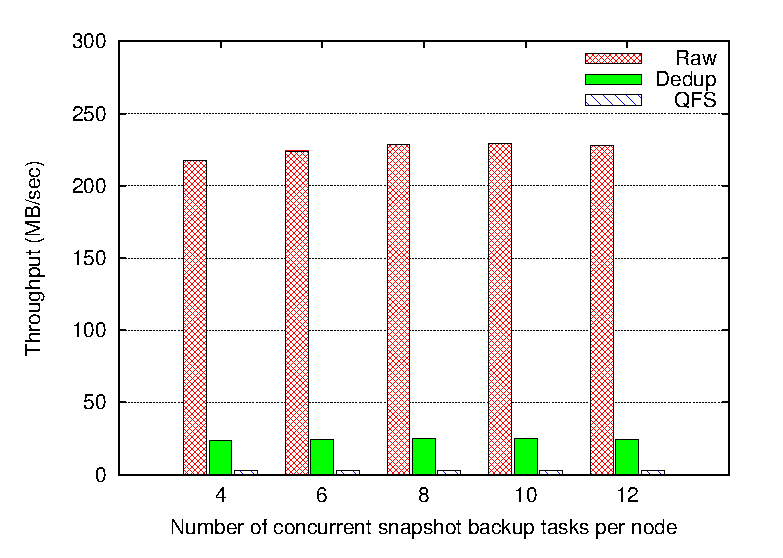
\includegraphics[width=3in]{figures/parallel_backup_with_read}
%         \label{fig:withread}
%     }
%     \\
%     \subfigure[Deduplication and storage system performance]
%     {
%         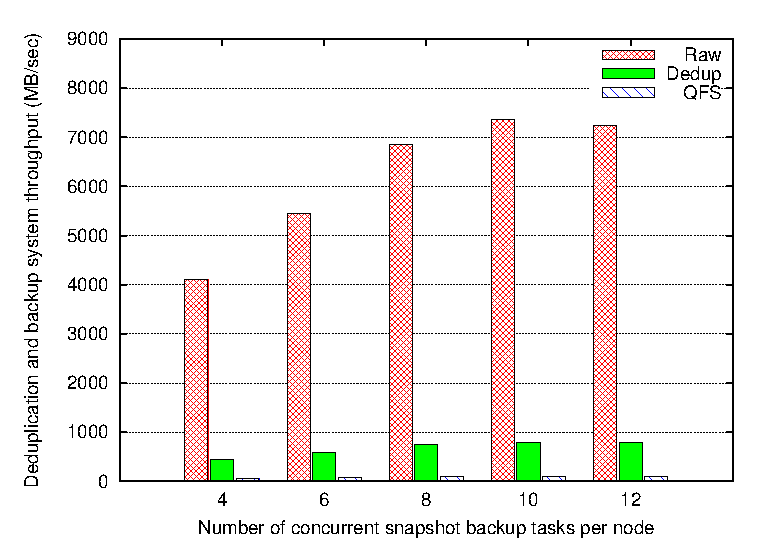
\includegraphics[width=3in]{figures/parallel_backup_no_read}
%         \label{fig:noread}
%     }
%     \caption{Throughput per-node with concurrent snapshot backup tasks}
%     \label{fig:parallel_backup}
% \end{figure}

 \subsection{Effectiveness of Approximate Deletion}
 \begin{figure}
     \centering
     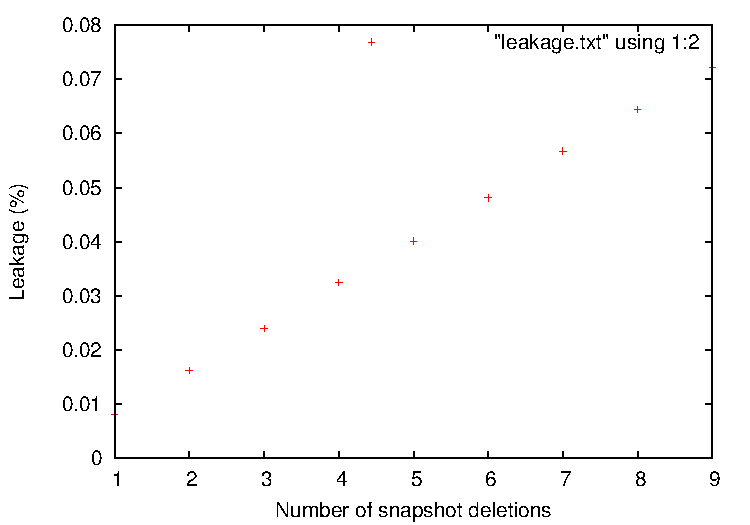
\includegraphics[width=3in]{figures/leakage}
     \caption{Accumulated storage leakage by approximate snapshot deletions}
     \label{fig:leakage}
 \end{figure}

Figure~\ref{fig:leakage} shows the average accumulated storage leakage in terms of percentage of
storage space per VM caused  by approximate deletions.
The solid line is the predicted leakage using Formula~\ref{eq:leakrepair} from Section~\ref{sect:delete}
while the dashed line is the actual leakage measured during the experiment.
% [OTHER PARAMETERS USED]
After 9 snapshot deletions, the actual leakage reaches 0.01\% and this means that
there is only 1MB space leaked for every 10GB of stored data. 

\section{Conclusion}
\label{sect:final}
In this paper we propose a collocated backup service built on
the top of a cloud cluster to reduce network traffic and infrastructure.
The key contribution is a VM-centric deduplication scheme to 
maximize fault isolation while delivering competitive deduplication efficiency.
Inner-VM deduplication localizes backup data dependency and exposes more parallelism  
while cross-VM deduplication with a small common data set.
VM-specific file block packing also reduces inter-VM dependence and enhances fault tolerance.
The design places a special consideration for low-resource usages as a collocated cloud service.
Evaluation using  VM backup data shows that
our solution can accomplish 92\% of what complete global
deduplication can do while the availability of snapshots increases substantially with this VM-centric
and a small replication overhead for popular inter-VM chunks.


\bibliographystyle{abbrv}
\bibliography{library,dedup1}
\end{document}
